\textit{Note on Group Work: This project was initially started as a group of two. However, my partner decided to withdraw during the development process, citing insufficient time to complete both this project and assignments from other courses. Consequently, the entirety of the implementation and advanced features presented in this report were completed individually.}

\section{Introduction}

As part of the INFO0004-2 project, I developed \textit{Carré Surfer}, a C++ endless runner game. The player takes on the role of Thomas, a student walking through the "Carré" district in Liège, who must avoid various obstacles while trying to get back home.

The objective of this project was to put into practice the object-oriented programming concepts covered in class, including inheritance, polymorphism, and rigorous memory management. I also aimed to enhance the gaming experience by adding advanced features, including an autonomous artificial intelligence.

\begin{figure}[H]
    \centering
    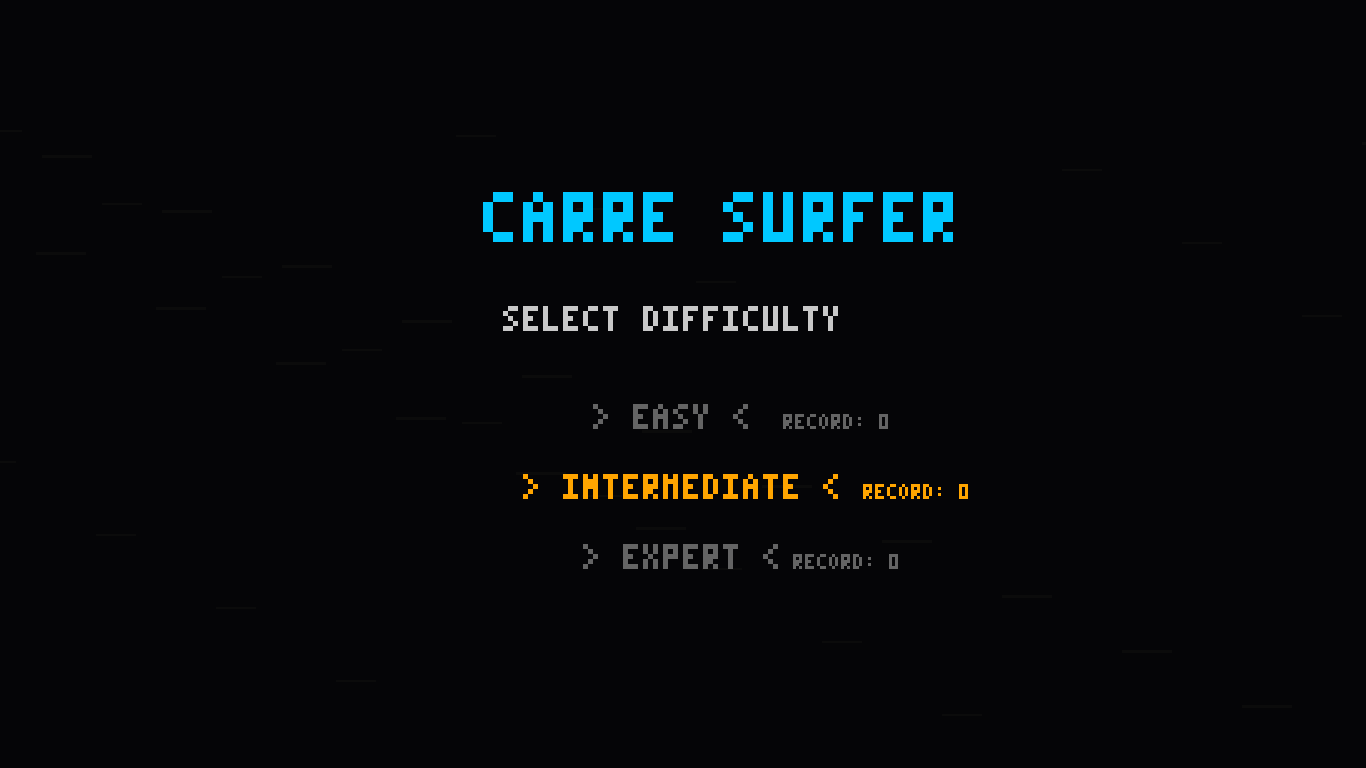
\includegraphics[width=0.6\textwidth]{images/home_screen.png}
    \caption{Game home screen showing the different difficulty modes.}
\end{figure}
